\chapter{Evaluation of the measured data}

The first step is to copy the data from the SD-Card into an empty folder. 
Then one can start the \script{CompEval.py}, which opens the window shown in Fig. \ref{fig:mainWindow_Evaluation}. After pressing the button "Process Raw Data" a file selection window is opened, in which the recently saved files should be selected. This step may take a while, dependent on the file count and file size (The window may not react during this process). 

Afterwards a second file selection window will be opened, where the splitted and smoothed data should be selected (e.g. by pressing "Ctrl+A"). 


As soon as both steps are finished, the button "Process Raw Data" will turn green and one can let the software calculate the thicknesses of the measurement data by pressing "Get Thicknesses". 
In the opened file selection window you need to select the measurement data of the first laser (called "green" laser), in the second file selection window the data of the second laser (called "red" laser). 


Now the window shown in Fig. \ref{fig:thickness_parameters} will open, here the correct parameters need to be inserted. After pressing "Start" the thicknesses will be calculated and saved. 

By pressing the button "Start Evaluation" one can select the "Result-Files" and evaluate the data with the windows shown in Figs. \ref{fig:evaluation_plot} and \ref{fig:evaluation_control}.

One can use the buttons in Fig. \ref{fig:evaluation_control} for selecting the measurement points, which should be fitted. Another method is to use the keyboard buttons (after clicking in the empty text field), shown in Tab. \ref{tab:shortcuts}. 

By pressing "List Selection" a window (Fig. \ref{fig:evaluation_selection}) is opened, where all confirmed points are shown. Here one can delete points, e.g. after selecting them accidentally. 
In this window one can press "Show Selection" to show all selected points in the plot.

The button "Start automatic selection" will select all points, which are one step below the last confirmed point. 


\begin{figure}
	\centering
	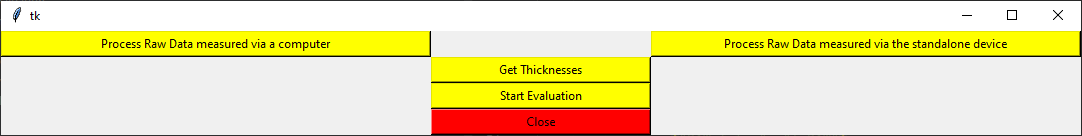
\includegraphics[width=0.7\linewidth]{LamellaDevice_Evaluation/Software}
	\caption{Screenshot of the main window of the evaluation software.}
	\label{fig:mainWindow_Evaluation}
\end{figure}

\begin{figure}
	\centering
	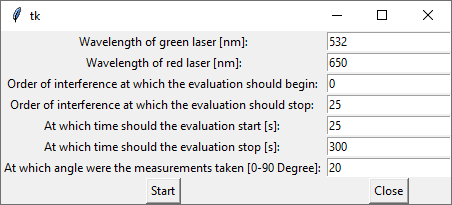
\includegraphics[width=0.7\linewidth]{LamellaDevice_Evaluation/Parameters}
	\caption{Screenshot of the parameters for fitting the data.}
	\label{fig:thickness_parameters}
\end{figure}

\begin{figure}
	\centering
	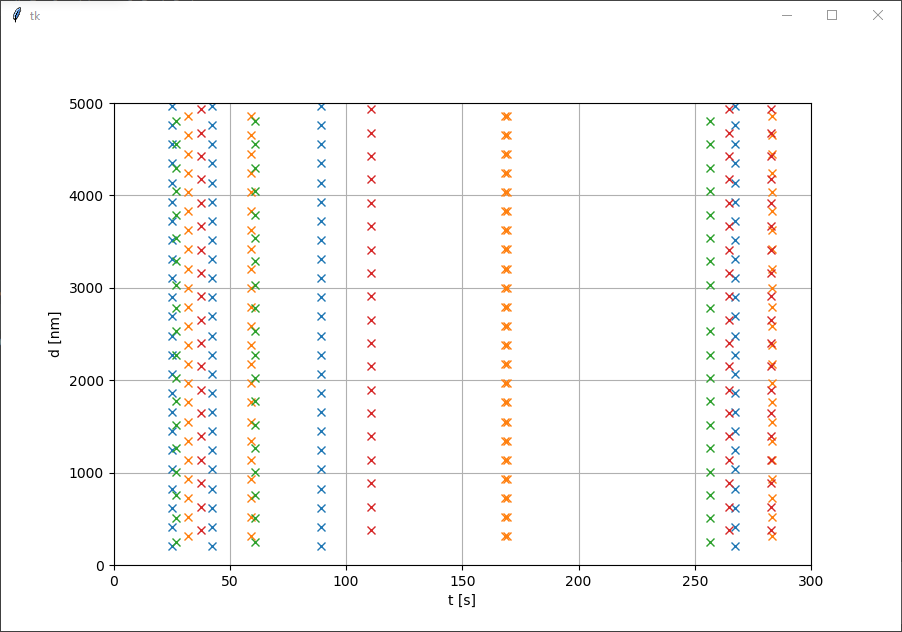
\includegraphics[width=0.7\linewidth]{LamellaDevice_Evaluation/Evaluation_Plot}
	\caption{Screenshot of the plot during evaluation.}
	\label{fig:evaluation_plot}
\end{figure}

\begin{figure}
	\centering
	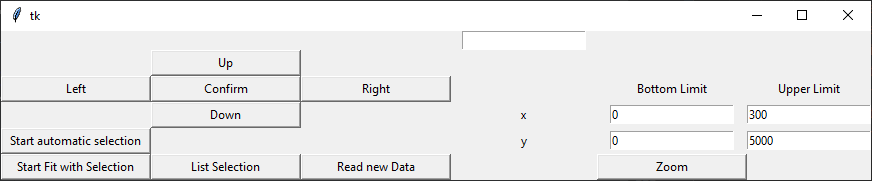
\includegraphics[width=0.7\linewidth]{LamellaDevice_Evaluation/Evaluation_Control}
	\caption{Screenshot of the control window during evaluation.}
	\label{fig:evaluation_control}
\end{figure}

\begin{table}
	\centering
	\caption{Buttons as shortcuts for the control-functions.}
	\label{tab:shortcuts}
	\begin{tabular}{|c|c|}
		\hline
		Button & Function \\
		\hline
		W & Upwards \\
		\hline
		S & Down \\
		\hline
		A & Left \\
		\hline
		D & Right \\
		\hline
		C & Confirm \\
		\hline
	\end{tabular}
\end{table}

\begin{figure}
	\centering
	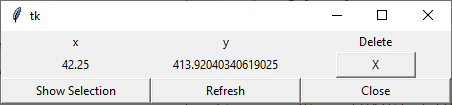
\includegraphics[width=0.7\linewidth]{LamellaDevice_Evaluation/Evaluation_Selection}
	\caption{Screenshot, in which the selected points are shown.}
	\label{fig:evaluation_selection}
\end{figure}

\begin{figure}
	\centering
	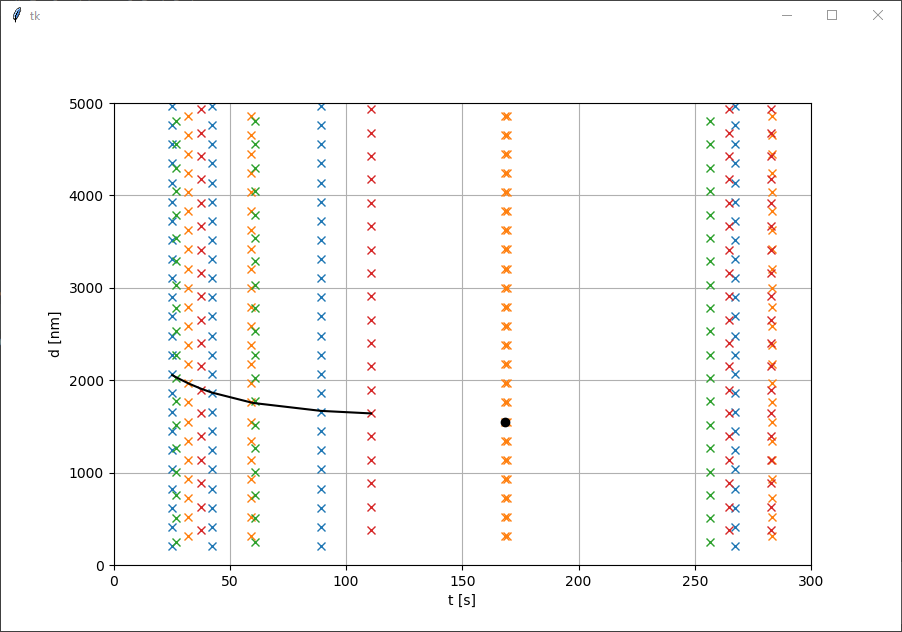
\includegraphics[width=0.7\linewidth]{LamellaDevice_Evaluation/Evaluation_Fitted}
	\caption{Screenshot of the plot after fitting the confirmed measurement points. }
	\label{fig:evaluation_fitted}
\end{figure}

\begin{figure}
	\centering
	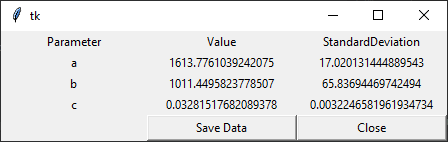
\includegraphics[width=0.7\linewidth]{LamellaDevice_Evaluation/Evaluation_Results}
	\caption{Screenshot of the result window after fitting the measurement points.}
	\label{fig:evaluation_results}
\end{figure}
